\begin{frame}{曲率}
	\linespread{1.2}
	\centerline{\ba{如何刻画曲线的弯曲程度?}}
	\pause
	\begin{columns}
		\column{.5\textwidth}
			\begin{center}
				\vspace{-1em}
				{\resizebox{!}{5.5cm}{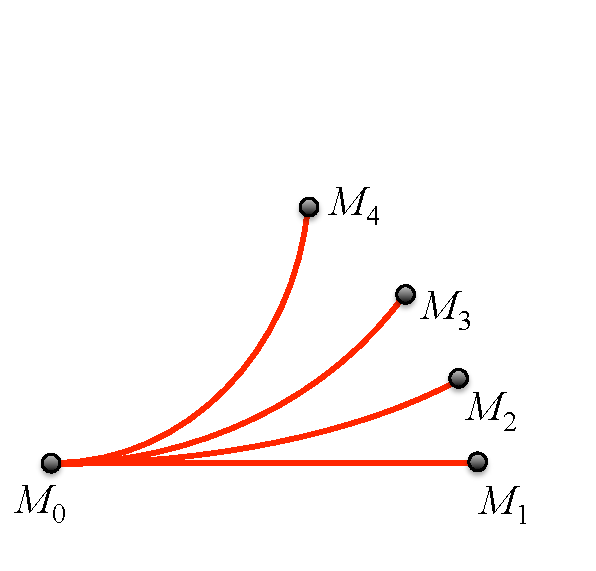
\includegraphics{./images/curves/c106.pdf}}}

				\vspace{-1em}\invisible<1->{{\b 长度相同的曲线,切线

				转角越大弯曲程度越大}}
			\end{center}
		\column{.5\textwidth}
	\end{columns}
\end{frame}

\begin{frame}{曲率}
	\linespread{1.2}
	\centerline{\ba{如何刻画曲线的弯曲程度?}}

	\begin{columns}
		\column{.5\textwidth}
			\begin{center}
				\vspace{-1em}
				{\resizebox{!}{5.5cm}{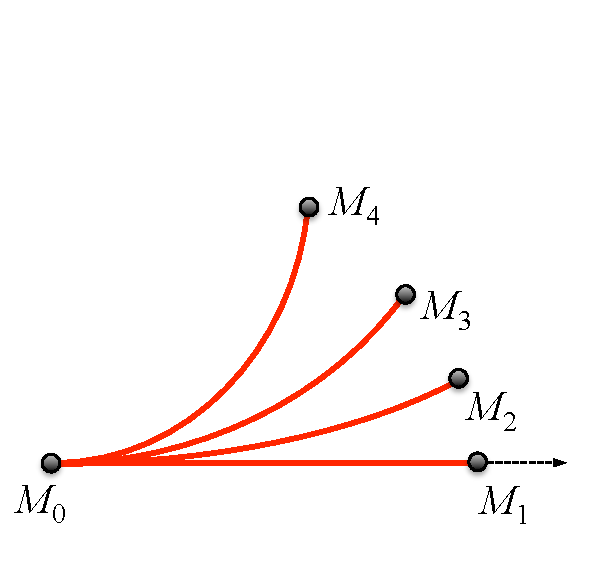
\includegraphics{./images/curves/c105.pdf}}}

				\vspace{-1em}\invisible<1->{{\b 长度相同的曲线,切线

				转角越大弯曲程度越大}}
			\end{center}
		\column{.5\textwidth}
	\end{columns}
\end{frame}

\begin{frame}{曲率}
	\linespread{1.2}
	\centerline{\ba{如何刻画曲线的弯曲程度?}}

	\begin{columns}
		\column{.5\textwidth}
			\begin{center}
				\vspace{-1em}
				{\resizebox{!}{5.5cm}{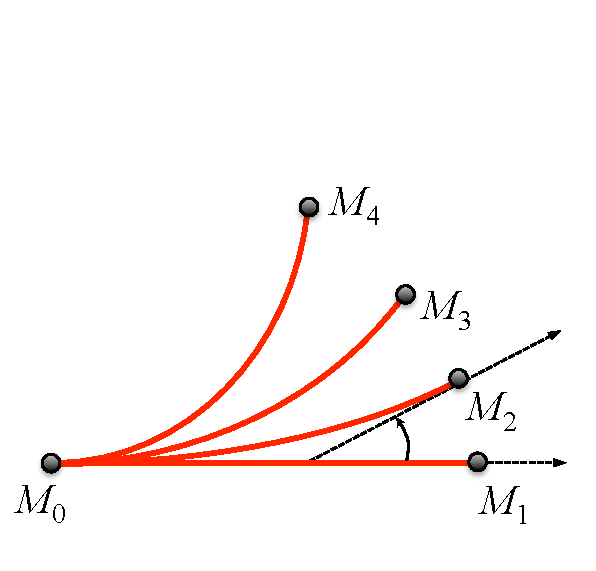
\includegraphics{./images/curves/c104.pdf}}}

				\vspace{-1em}\invisible<1->{{\b 长度相同的曲线,切线

				转角越大弯曲程度越大}}
			\end{center}
		\column{.5\textwidth}
	\end{columns}
\end{frame}

\begin{frame}{曲率}
	\linespread{1.2}
	\centerline{\ba{如何刻画曲线的弯曲程度?}}

	\begin{columns}
		\column{.5\textwidth}
			\begin{center}
				\vspace{-1em}
				{\resizebox{!}{5.5cm}{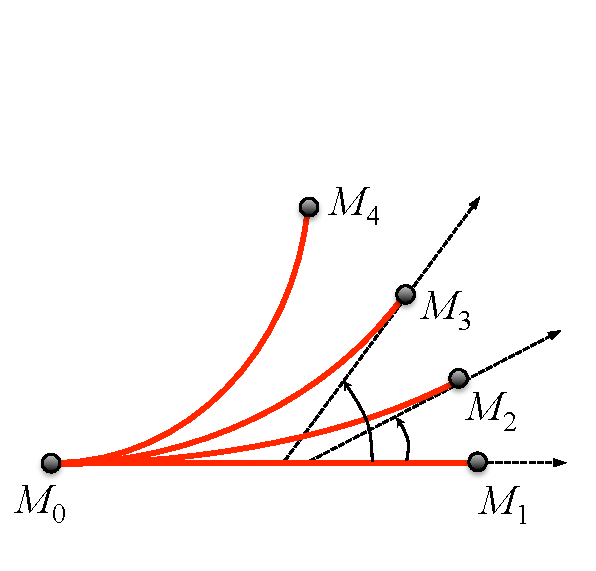
\includegraphics{./images/curves/c103.pdf}}}

				\vspace{-1em}\invisible<1->{{\b 长度相同的曲线,切线

				转角越大弯曲程度越大}}
			\end{center}
		\column{.5\textwidth}
	\end{columns}
\end{frame}

\begin{frame}{曲率}
	\linespread{1.2}
	\centerline{\ba{如何刻画曲线的弯曲程度?}}

	\begin{columns}
		\column{.5\textwidth}
			\begin{center}
				\vspace{-1em}
				{\resizebox{!}{5.5cm}{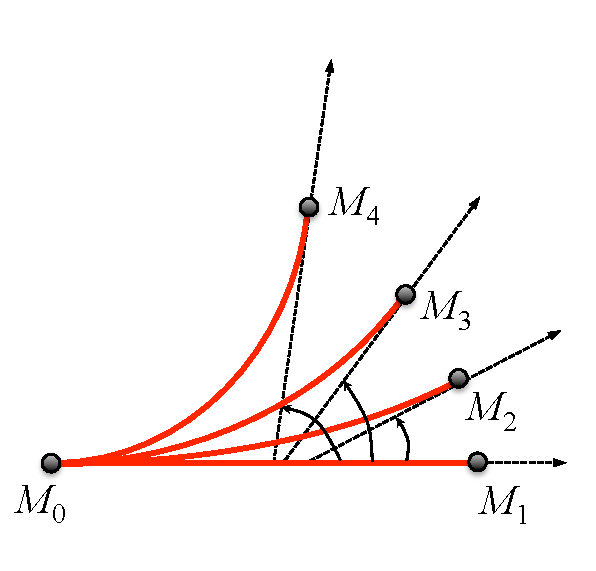
\includegraphics{./images/curves/c102.pdf}}}

				\vspace{-1em}\invisible<1->{{\b 长度相同的曲线,切线

				转角越大弯曲程度越大}}
			\end{center}
		\column{.5\textwidth}
	\end{columns}
\end{frame}

\begin{frame}{曲率}
	\linespread{1.2}
	\centerline{\ba{如何刻画曲线的弯曲程度?}}

	\begin{columns}
		\column{.5\textwidth}
			\begin{center}
				\vspace{-1em}
				{\resizebox{!}{5.5cm}{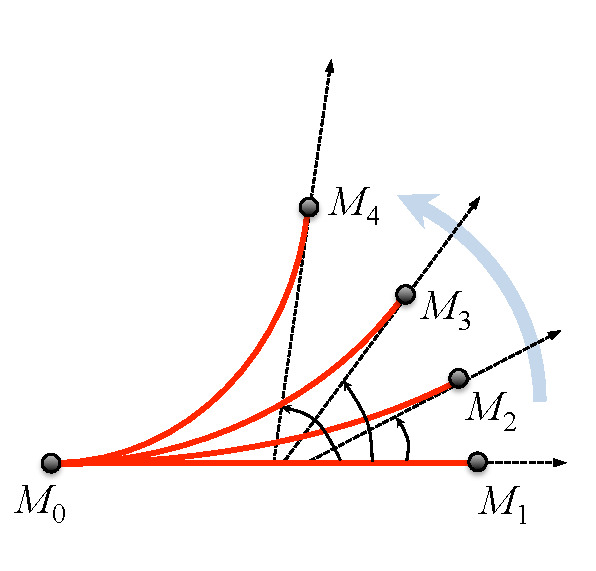
\includegraphics{./images/curves/c101.pdf}}}

				\vspace{-1em}{{\b 长度相同的曲线,切线

				转角越大弯曲程度越大}}
			\end{center}
		\column{.5\textwidth}
	\end{columns}
\end{frame}

% \begin{frame}{曲率}
% 	\linespread{1.2}
% 	\centerline{\ba{如何刻画曲线的弯曲程度?}}
% 
% 	\begin{columns}
% 		\column{.5\textwidth}
% 			\begin{center}
% 				\vspace{-1em}
% 				{\resizebox{!}{5.5cm}{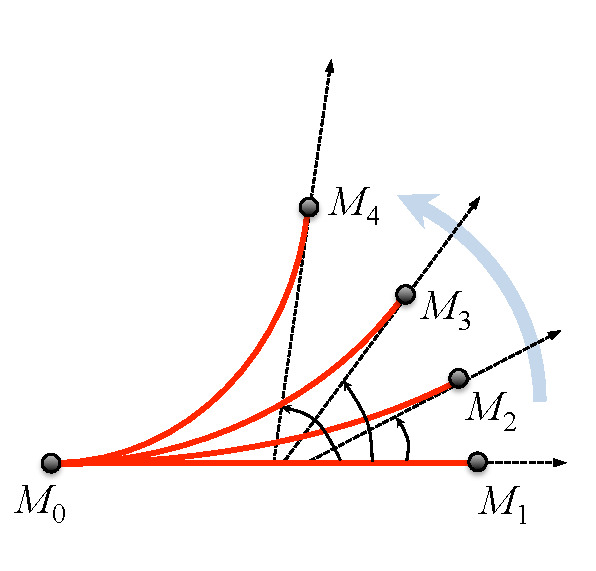
\includegraphics{./images/curves/c101.pdf}}}
% 
% 				\vspace{-1em}{{\b 长度相同的曲线,切线
% 				
% 				转角越大弯曲程度越大}}	
% 			\end{center}
% 		\column{.5\textwidth}
% 			\begin{center}			
% 				\vspace{-1em}
% 				{\resizebox{!}{5.5cm}{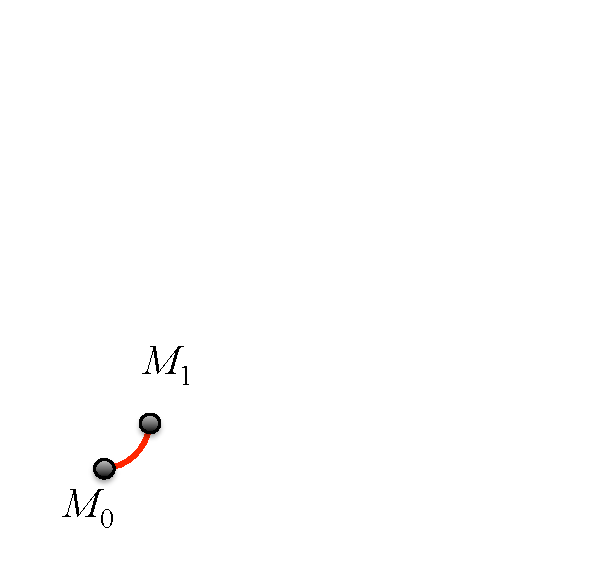
\includegraphics{./images/curves/c208.pdf}}}
% 				
% 				\vspace{-1em}{\color{white} 切线转角相同的曲线,
% 
% 				弧长越短弯曲程度越大}
% 			\end{center}
% 	\end{columns}
% \end{frame}
% 
% \begin{frame}{曲率}
% 	\linespread{1.2}
% 	\centerline{\ba{如何刻画曲线的弯曲程度?}}
% 
% 	\begin{columns}
% 		\column{.5\textwidth}
% 			\begin{center}
% 				\vspace{-1em}
% 				{\resizebox{!}{5.5cm}{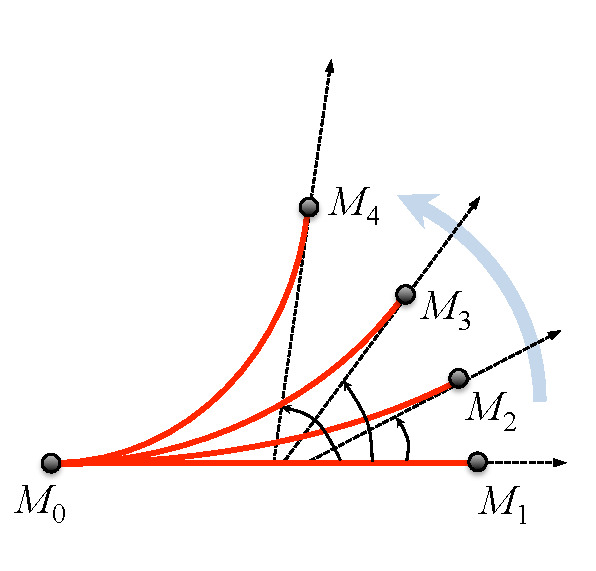
\includegraphics{./images/curves/c101.pdf}}}
% 
% 				\vspace{-1em}{{\b 长度相同的曲线,切线
% 
% 				转角越大弯曲程度越大}}
% 			\end{center}
% 		\column{.5\textwidth}
% 			\begin{center}
% 				\vspace{-1em}
% 				{\resizebox{!}{5.5cm}{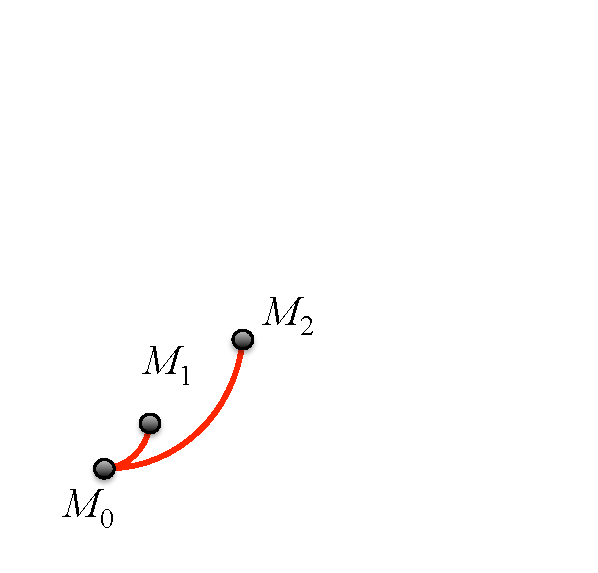
\includegraphics{./images/curves/c207.pdf}}}
% 				
% 				\vspace{-1em}{\color{white} 切线转角相同的曲线,
% 
% 				弧长越短弯曲程度越大}
% 			\end{center}
% 	\end{columns}
% \end{frame}

\begin{frame}{曲率}
	\linespread{1.2}
	\centerline{\ba{如何刻画曲线的弯曲程度?}}

	\begin{columns}
		\column{.5\textwidth}
			\begin{center}
				\vspace{-1em}
				{\resizebox{!}{5.5cm}{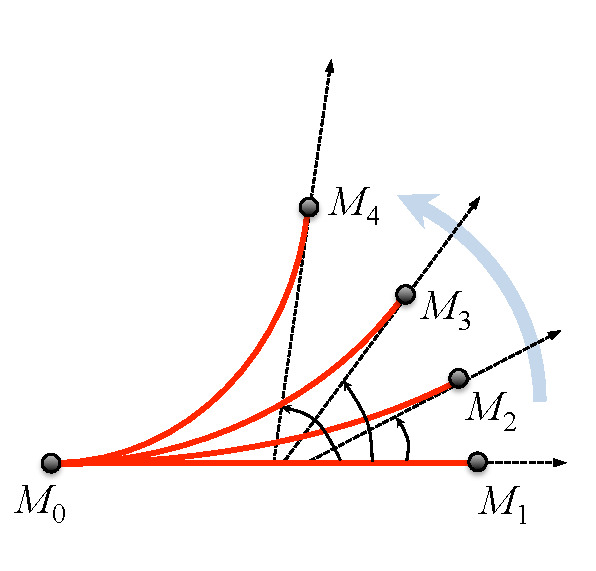
\includegraphics{./images/curves/c101.pdf}}}

				\vspace{-1em}{{\b 长度相同的曲线,切线

				转角越大弯曲程度越大}}
			\end{center}
		\column{.5\textwidth}
			\begin{center}
				\vspace{-1em}
				{\resizebox{!}{5.5cm}{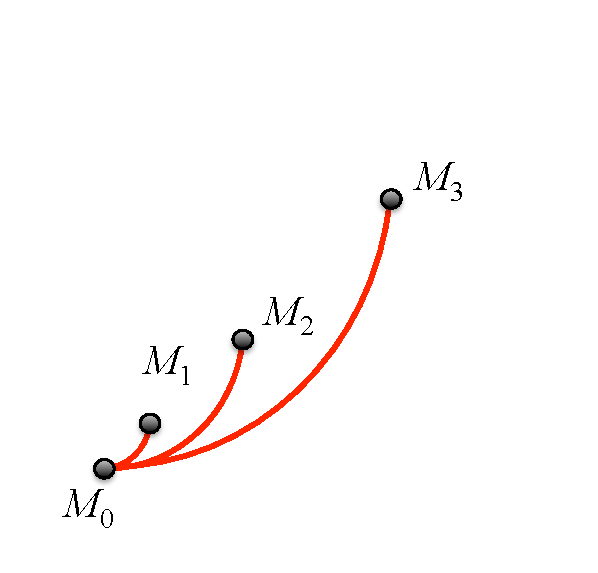
\includegraphics{./images/curves/c206.pdf}}}
				
				\vspace{-1em}{\color{white} 切线转角相同的曲线,

				弧长越短弯曲程度越大}
			\end{center}
	\end{columns}
\end{frame}

\begin{frame}{曲率}
	\linespread{1.2}
	\centerline{\ba{如何刻画曲线的弯曲程度?}}

	\begin{columns}
		\column{.5\textwidth}
			\begin{center}
				\vspace{-1em}
				{\resizebox{!}{5.5cm}{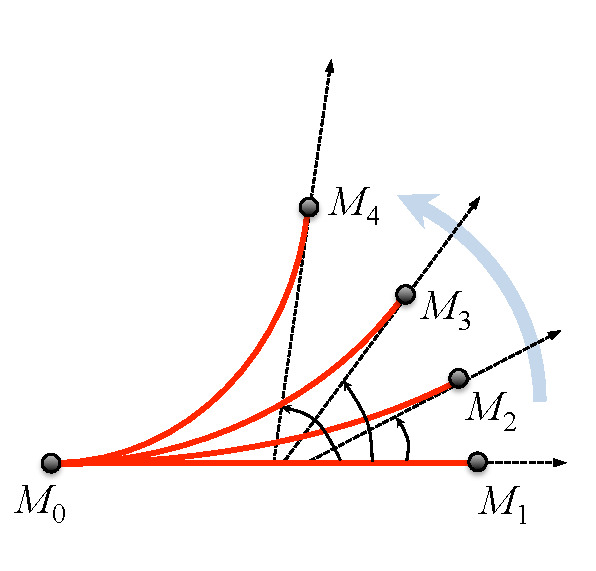
\includegraphics{./images/curves/c101.pdf}}}

				\vspace{-1em}{{\b 长度相同的曲线,切线

				转角越大弯曲程度越大}}
			\end{center}
		\column{.5\textwidth}
			\begin{center}
				\vspace{-1em}
				{\resizebox{!}{5.5cm}{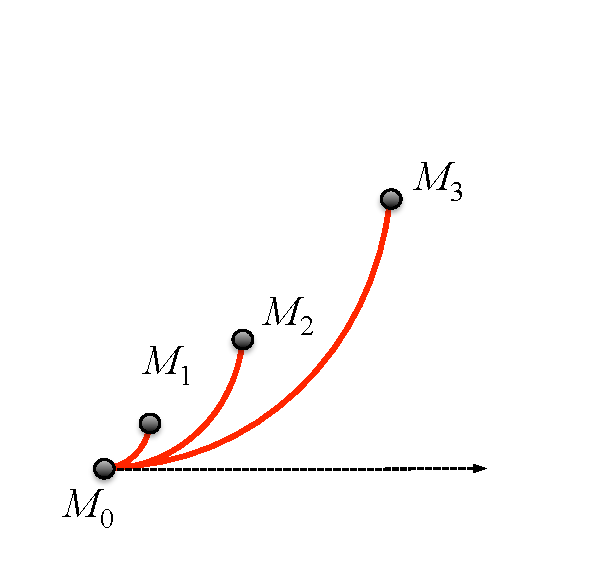
\includegraphics{./images/curves/c205.pdf}}}
				
				\vspace{-1em}{\color{white} 切线转角相同的曲线,

				弧长越短弯曲程度越大}
			\end{center}
	\end{columns}
\end{frame}

\begin{frame}{曲率}
	\linespread{1.2}
	\centerline{\ba{如何刻画曲线的弯曲程度?}}

	\begin{columns}
		\column{.5\textwidth}
			\begin{center}
				\vspace{-1em}
				{\resizebox{!}{5.5cm}{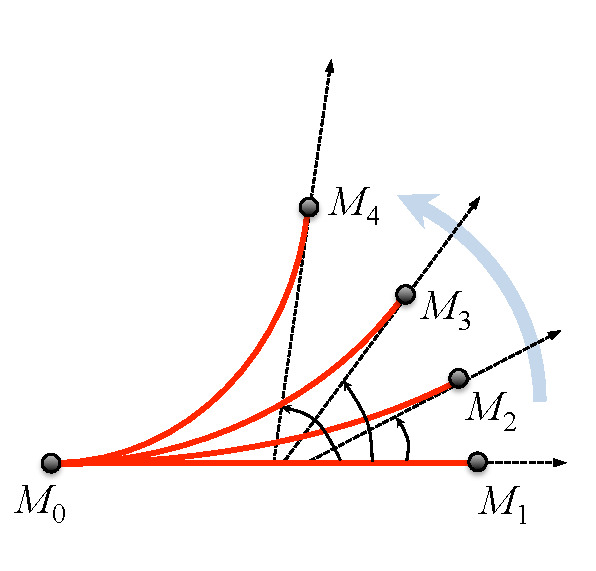
\includegraphics{./images/curves/c101.pdf}}}

				\vspace{-1em}{{\b 长度相同的曲线,切线

				转角越大弯曲程度越大}}
			\end{center}
		\column{.5\textwidth}
			\begin{center}
				\vspace{-1em}
				{\resizebox{!}{5.5cm}{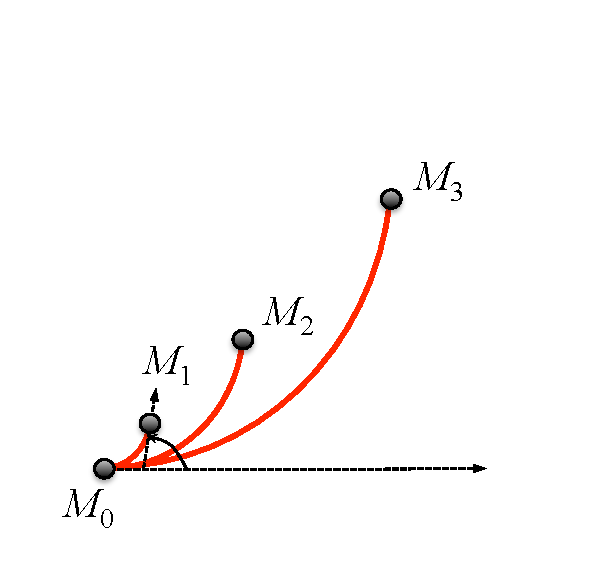
\includegraphics{./images/curves/c204.pdf}}}
				
				\vspace{-1em}{\color{white} 切线转角相同的曲线,

				弧长越短弯曲程度越大}
			\end{center}
	\end{columns}
\end{frame}

\begin{frame}{曲率}
	\linespread{1.2}
	\centerline{\ba{如何刻画曲线的弯曲程度?}}

	\begin{columns}
		\column{.5\textwidth}
			\begin{center}
				\vspace{-1em}
				{\resizebox{!}{5.5cm}{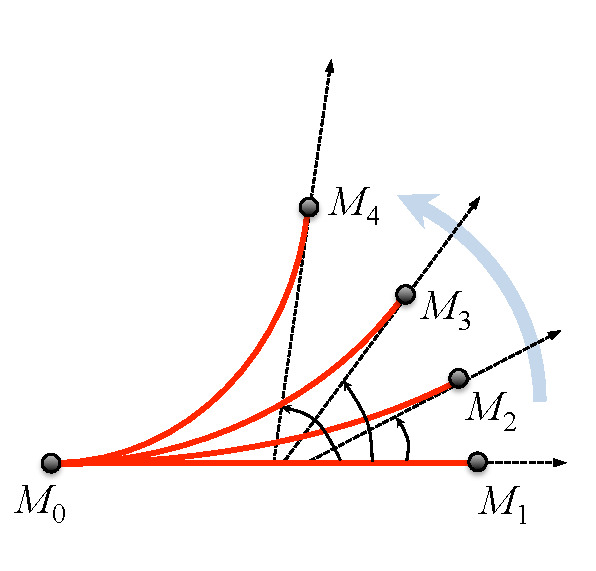
\includegraphics{./images/curves/c101.pdf}}}

				\vspace{-1em}{{\b 长度相同的曲线,切线

				转角越大弯曲程度越大}}
			\end{center}
		\column{.5\textwidth}
			\begin{center}
				\vspace{-1em}
				{\resizebox{!}{5.5cm}{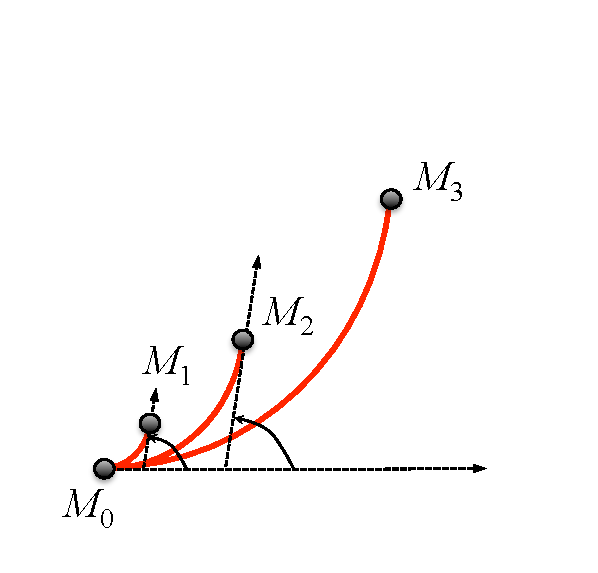
\includegraphics{./images/curves/c203.pdf}}}
				
				\vspace{-1em}{\color{white} 切线转角相同的曲线,

				弧长越短弯曲程度越大}
			\end{center}
	\end{columns}
\end{frame}

\begin{frame}{曲率}
	\linespread{1.2}
	\centerline{\ba{如何刻画曲线的弯曲程度?}}

	\begin{columns}
		\column{.5\textwidth}
			\begin{center}
				\vspace{-1em}
				{\resizebox{!}{5.5cm}{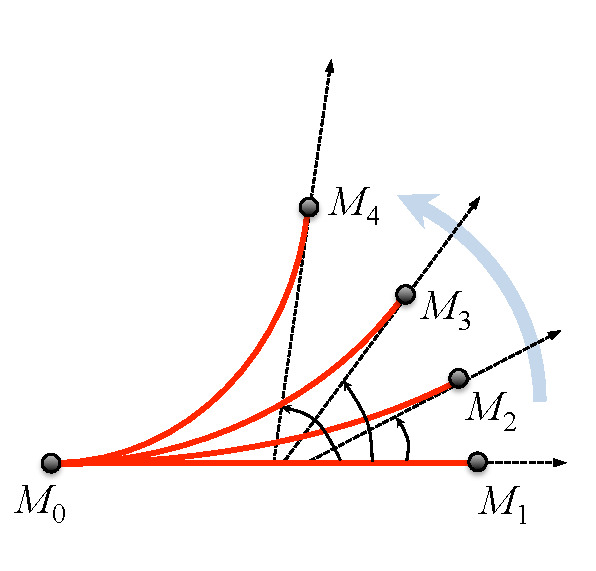
\includegraphics{./images/curves/c101.pdf}}}

				\vspace{-1em}{{\b 长度相同的曲线,切线

				转角越大弯曲程度越大}}
			\end{center}
		\column{.5\textwidth}
			\begin{center}
				\vspace{-1em}
				{\resizebox{!}{5.5cm}{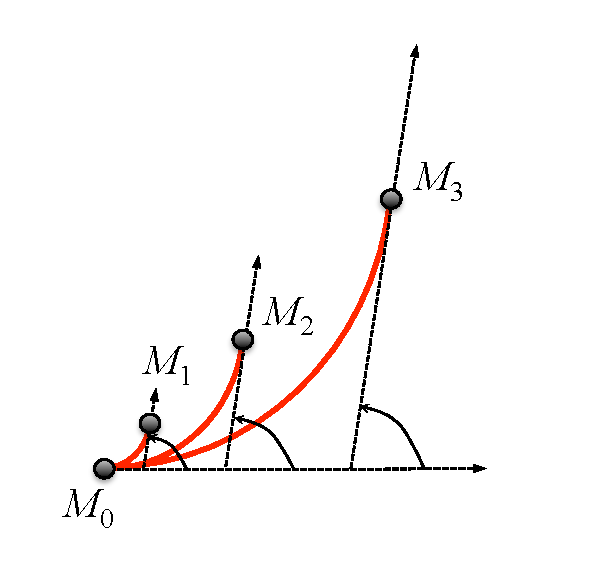
\includegraphics{./images/curves/c202.pdf}}}
				
				\vspace{-1em}{\color{white} 切线转角相同的曲线,

				弧长越短弯曲程度越大}
			\end{center}
	\end{columns}
\end{frame}

\begin{frame}{曲率}
	\linespread{1.2}
	\centerline{\ba{如何刻画曲线的弯曲程度?}}

	\begin{columns}
		\column{.5\textwidth}
			\begin{center}
				\vspace{-1em}
				{\resizebox{!}{5.5cm}{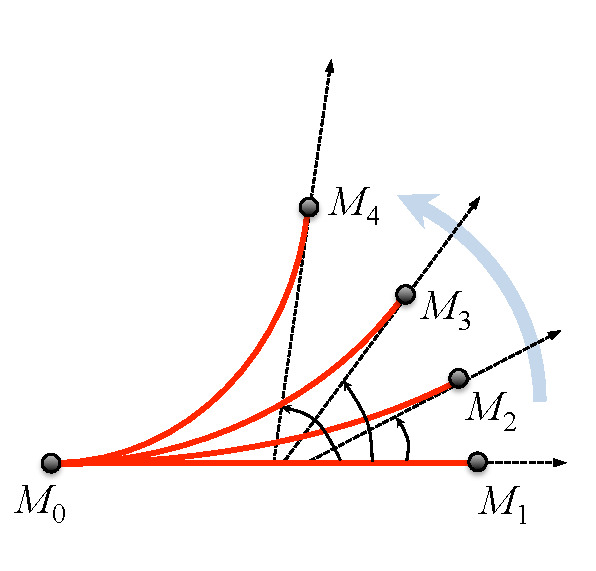
\includegraphics{./images/curves/c101.pdf}}}

				\vspace{-1em}{{\b 长度相同的曲线,切线

				转角越大弯曲程度越大}}
			\end{center}
		\column{.5\textwidth}
			\begin{center}
				\vspace{-1em}
				{\resizebox{!}{5.5cm}{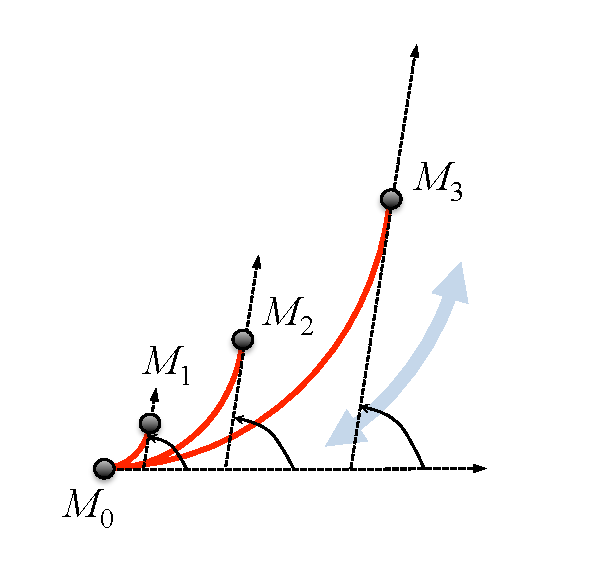
\includegraphics{./images/curves/c201.pdf}}}
				
				\vspace{-1em}{\b 切线转角相同的曲线,

				弧长越短弯曲程度越大}
			\end{center}
	\end{columns}
\end{frame}

%=================================================